\section{Analysis of the Experiment}
\label{sec:Auswertung}



\subsection{LED to Laserdiode}
\label{sec:LED_Laser}
First a threshold current of
\begin{align}
I_{\mathrm{threshold}} = \SI{}{\ampere}
\end{align}
is measured.
Futhermore in figure \ref{fig:threshold} the two
pictures from the camera focusing on the card are shown.
With the difference, that on one picture the current of the diode is below threshold \ref{fig:LED} and
on the other it is above threshold \ref{fig:LASER}.
\begin{figure}
  \centering
  \begin{subfigure}{0.45\textwidth}
    \centering
    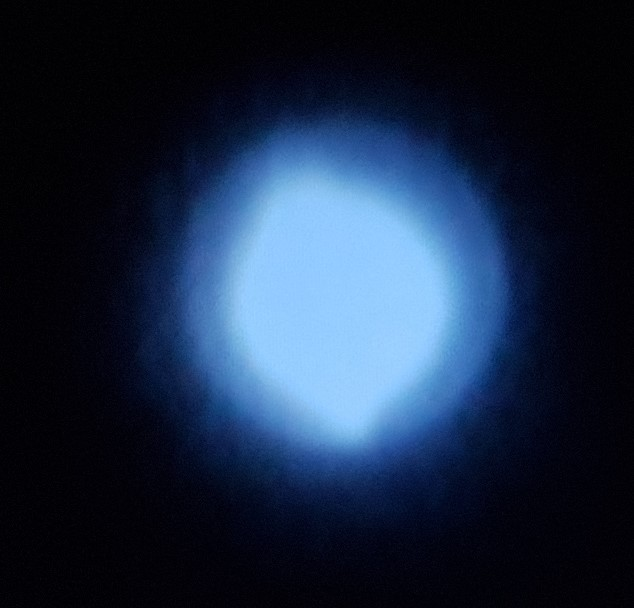
\includegraphics[height = 5cm]{figures/bevore_threshole.jpg}
    \caption{LED}
    \label{fig:LED}
  \end{subfigure}
  \begin{subfigure}{0.45\textwidth}
    \centering
    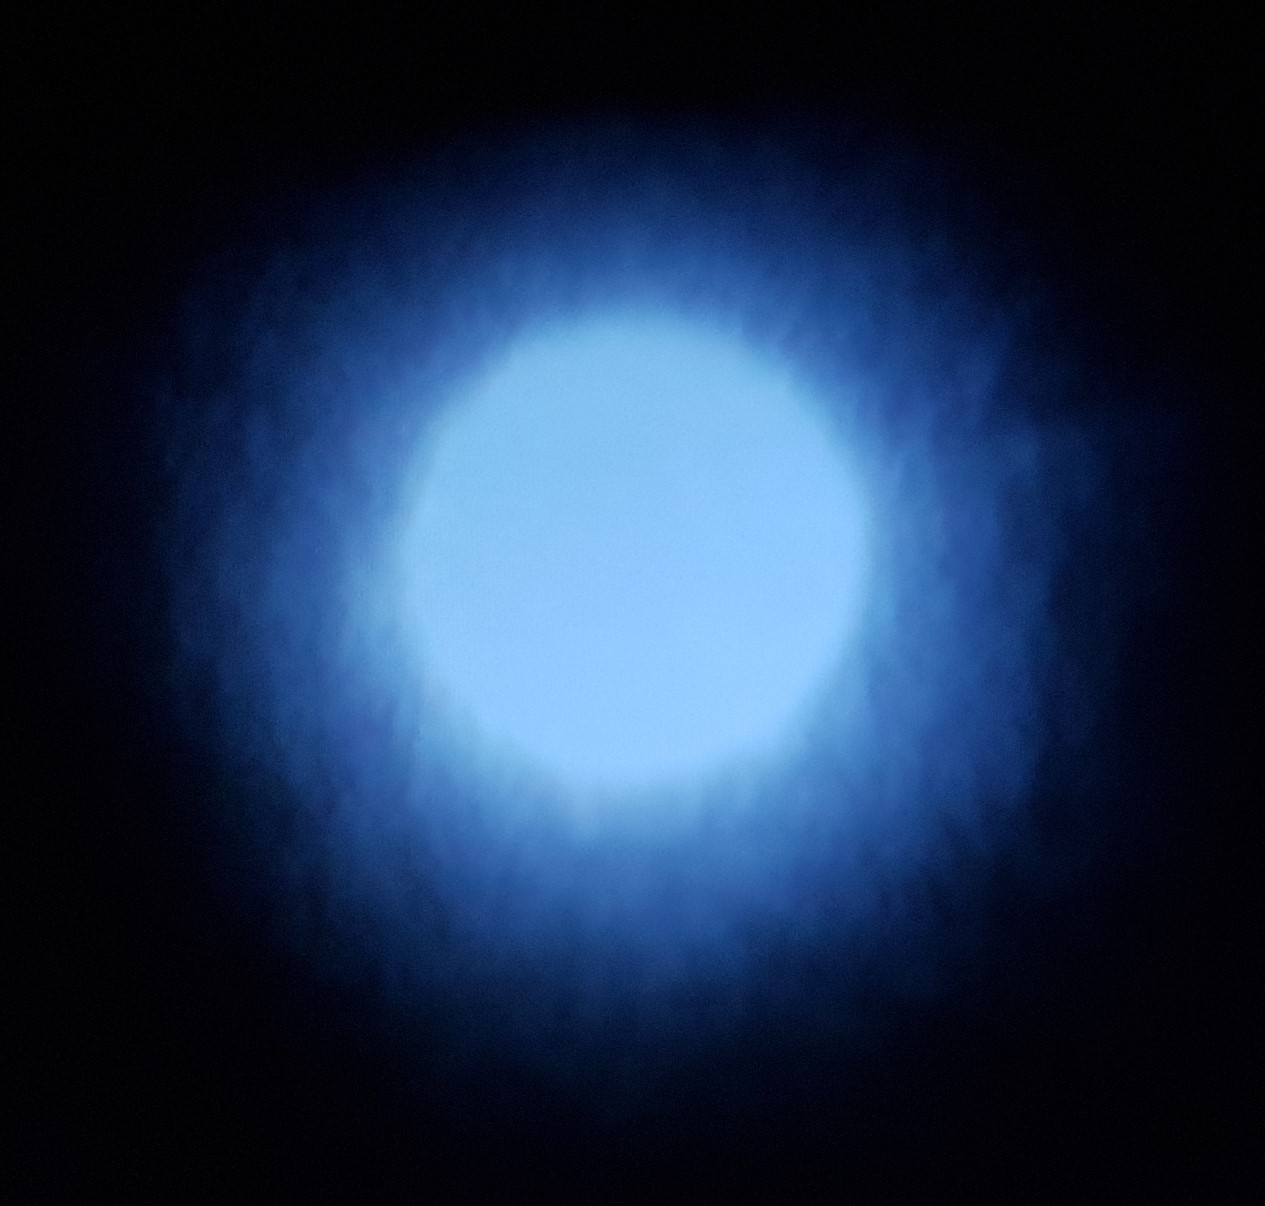
\includegraphics[height = 5cm]{figures/after_threshole.jpg}
    \caption{LASER}
    \label{fig:LASER}
  \end{subfigure}
\caption{The light below \ref{fig:LED} and above \ref{fig:LASER} the current threshold.}
\label{fig:threshold}
\end{figure}
The intensity change of the diode beam is clearly recognisable
between the lower intensity LED radiation \ref{fig:LED}
and the higher LASER radiation\ref{fig:LASER}.
% so the theory of a threshold current can be confirmed.

It follows the results for the setup \ref{fig:setup2}.
First with the rubidium absorption cell loceated in the laser beam
and the current adjusted so rubidium fluorescence is observed, the picture of the
camera, which is targeted at the
rubidium absorption cell, is
displayed in the figure \ref{fig:Floures}.

\begin{figure}
  \centering
  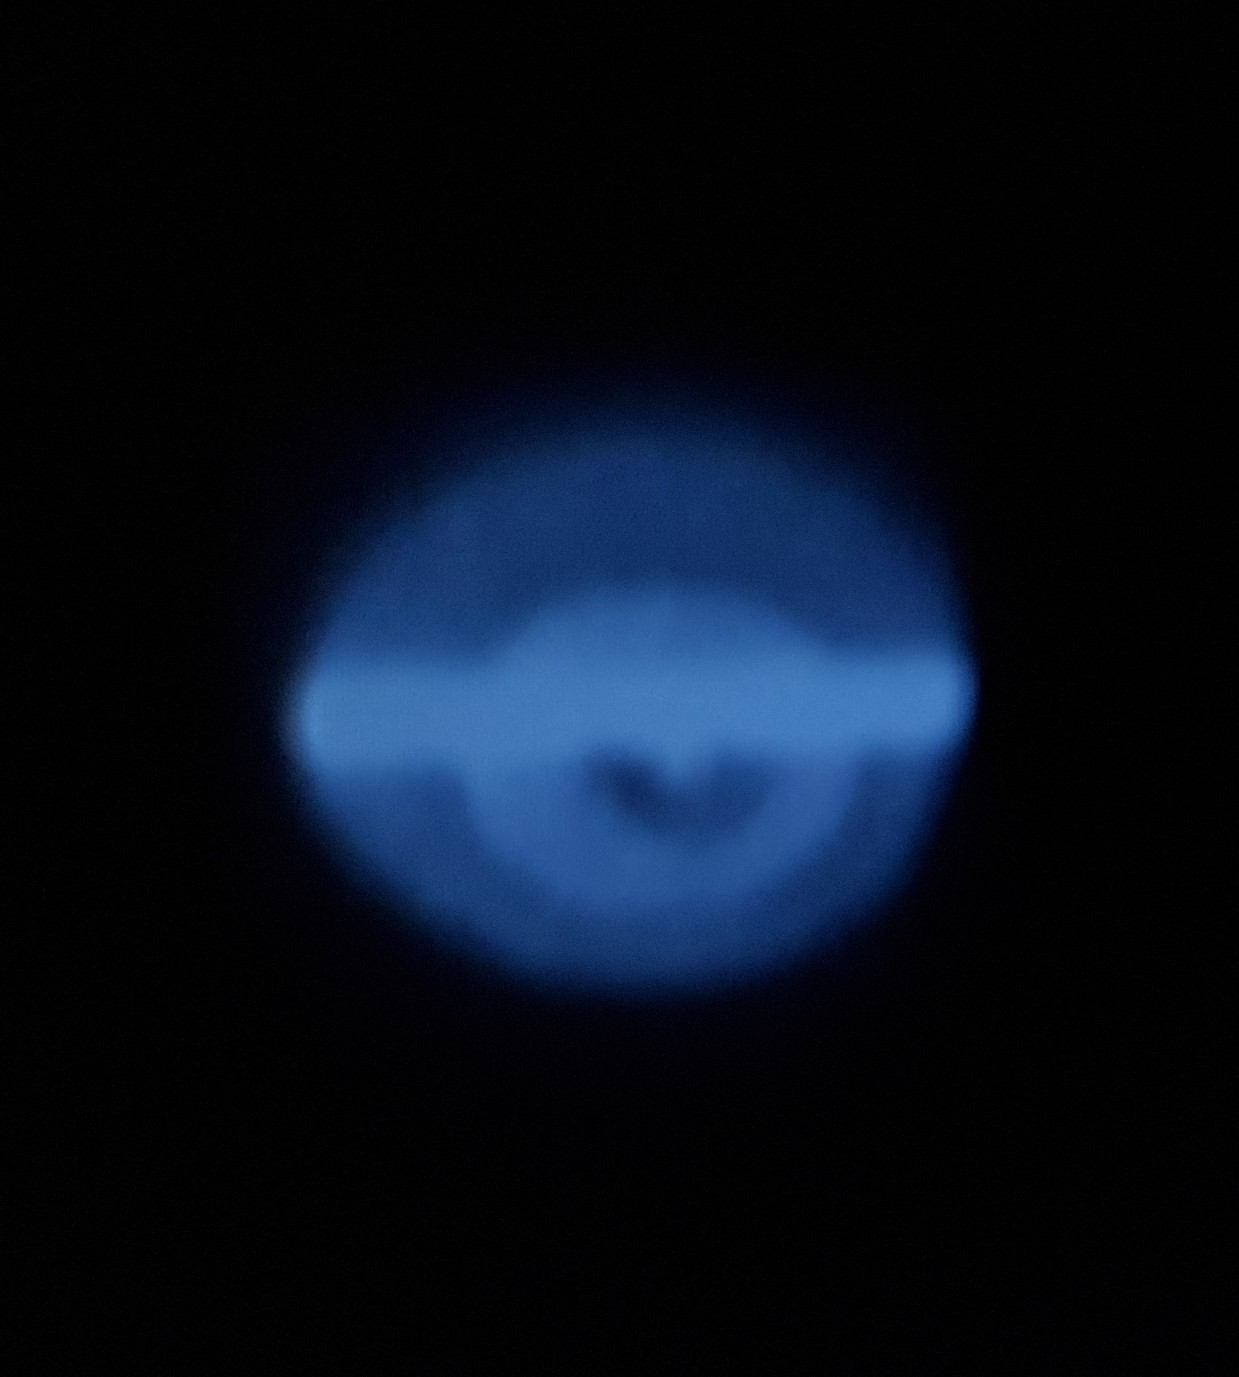
\includegraphics[width = 0.5\textwidth]{figures/Rb_leuchten.jpg}
  \caption{rubidium }
  \label{fig:Floures}
\end{figure}

rubidium flourescence is only observe in the Laser beam therfore
the brighter horizontal line
in figure \ref{fig:Floures}
is the track of the laser beam
goes through the rubidium cell and stimulates the rubidium atoms.

Now with the active ramp generator moving the grating with the piezo stack,
the signal from the photodiode behind the rubidium cell
is displayed with a
oscilloscope and shown in figure \ref{fig:ramp}.
Also the signal of the ramp generator is shown at the same
figure.

\begin{figure}
  \centering
  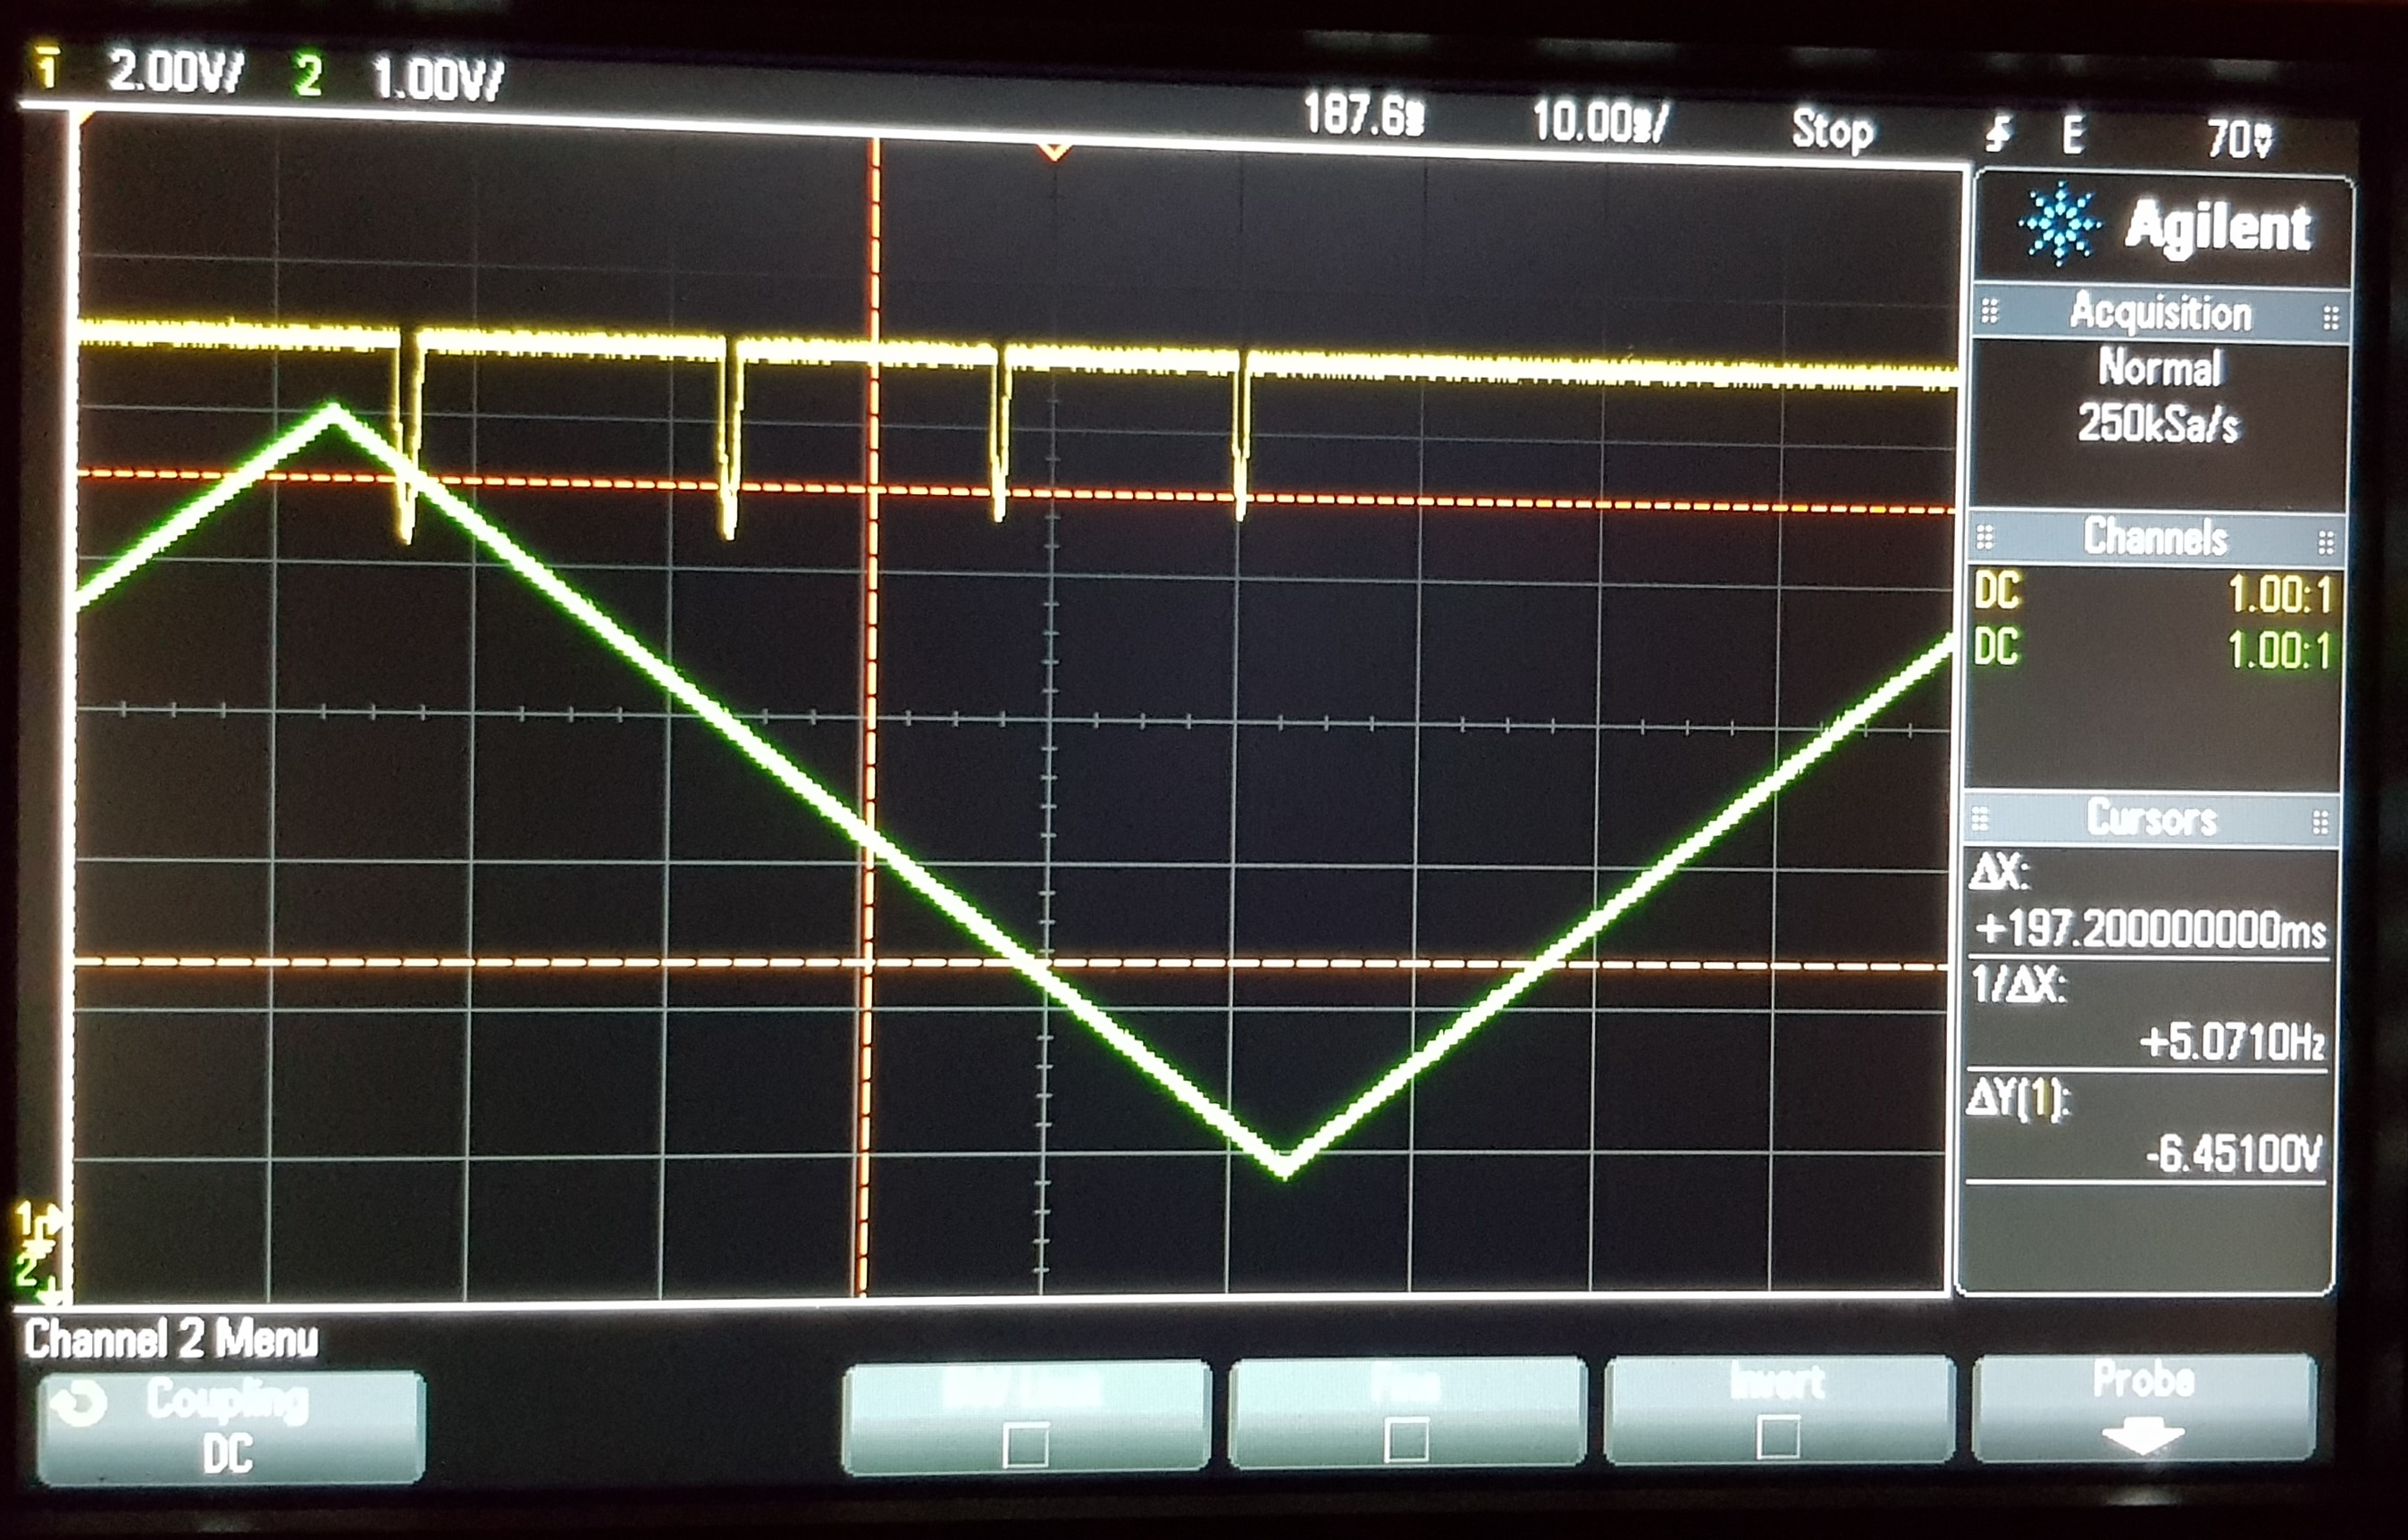
\includegraphics[width = 0.7\textwidth]{figures/Ramp.jpg}
  \caption{Signal from the photodiode and the ramp generator.}
  \label{fig:ramp}
\end{figure}

The figure \ref{fig:ramp} contains a part of the
absoptionspectrum as required.
For the rest of the measurements for the Rubidium absoptionspectrum
with only one photodiode, a problem with the storage medium
prevents further oscilloscope images.
But nevertheless
a image of scan over the hole Rubidium
with a simultaneous current and piezo modulation
can be produced. To get a impression of the possible image,
in figure \ref{fig:theory_curve} an example is displayed.

\begin{figure}
  \centering
  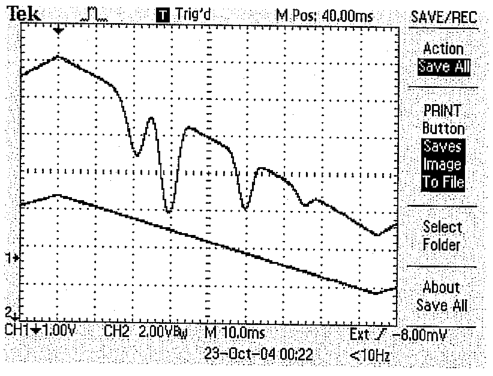
\includegraphics[width = 0.7\textwidth]{Rb_modulation.png}
  \caption{Signal from the photodiode and the ramp generator with
  simultaneous current and piezo modulation. \cite{V60}}
  \label{fig:theory_curve}
\end{figure}

Fortunately an oscilloscope image of the second measurement
with two Photodiodes
is available and displayed in figure \ref{fig:2dioden}.

\begin{figure}
  \centering
  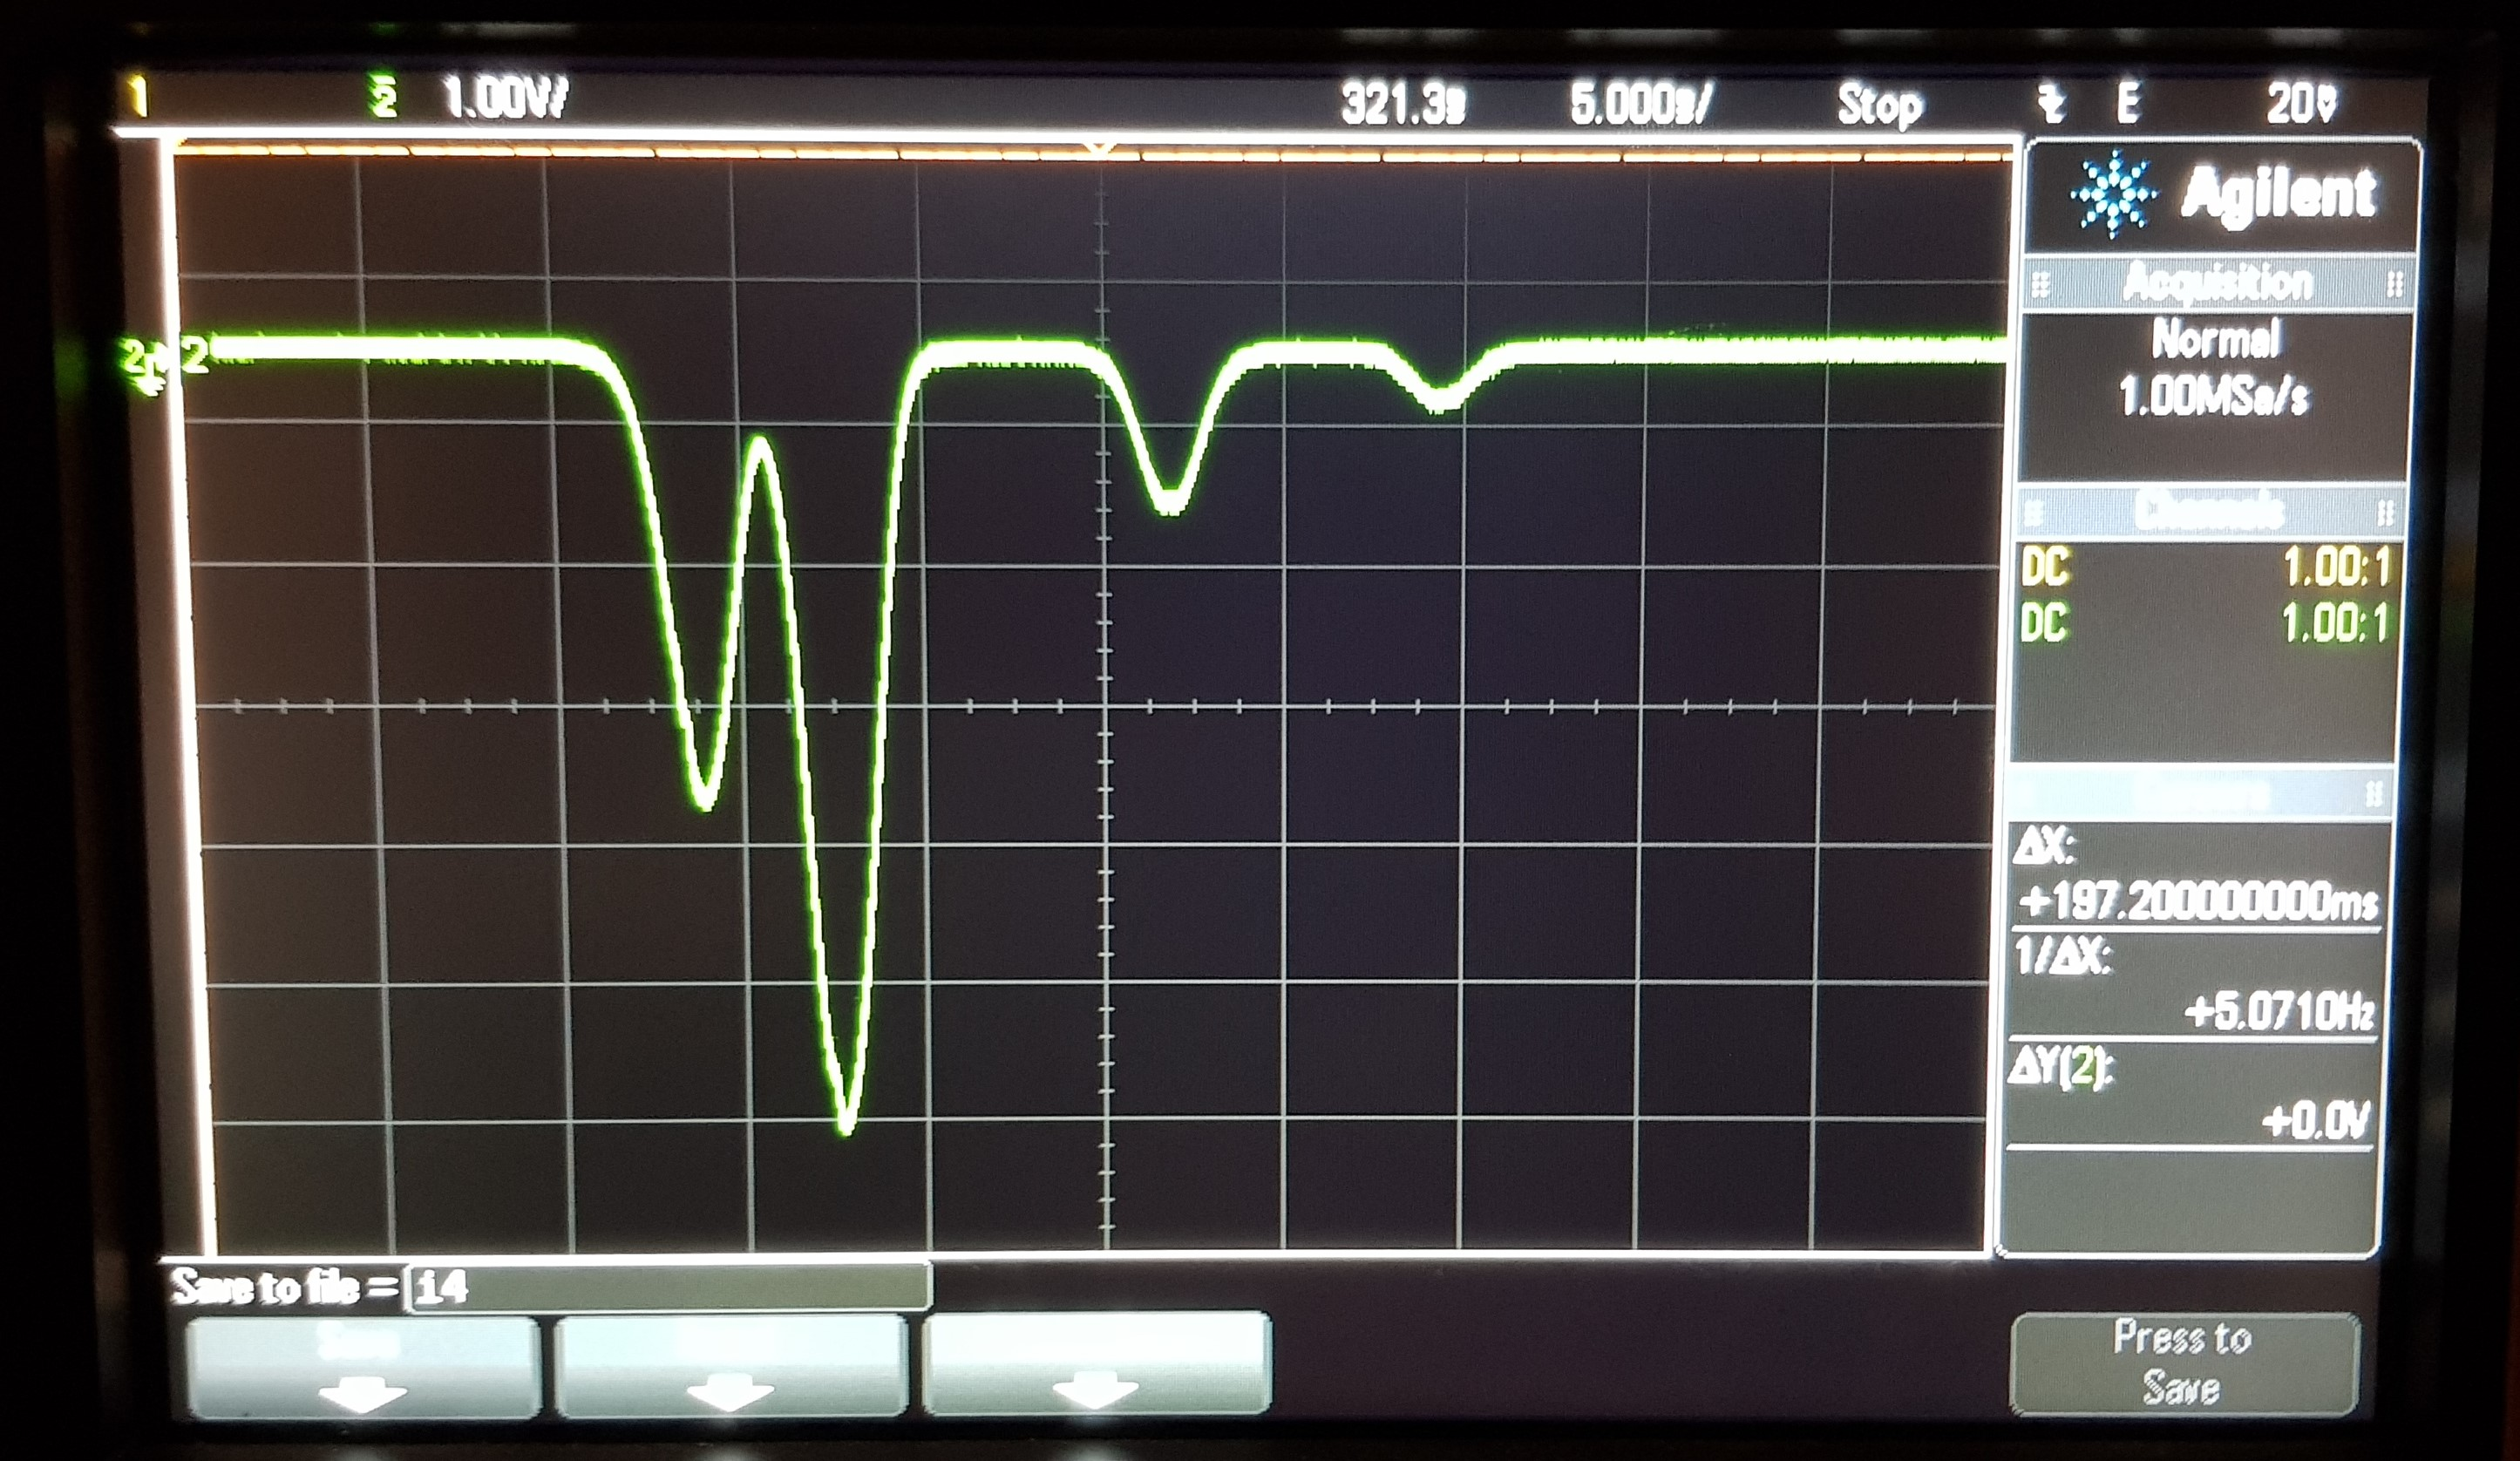
\includegraphics[width = 0.7\textwidth]{./figures/Rb_spectrum.jpg}
  \caption{Mix signal from the two photodiodes and aktive ramp generator with
  simultaneous current and piezo modulation.}
  \label{fig:2dioden}
\end{figure}

In contrast to the signal in figure \ref{fig:theory_curve}
the signal in figure \ref{fig:2dioden} the
ramp generator signal is not conntained in the mix signal anymore.
